\documentclass[border=4pt]{standalone}
\usepackage{fontspec}
\usepackage{amsmath}
\usepackage{unicode-math}
\setmainfont{Latin Modern Roman}
\setmathfont{Latin Modern Math}
\usepackage{pgfplots}
\usepackage{pgfplotstable}
\pgfplotsset{compat=1.18}
\usepackage{tkz-euclide}
\usetikzlibrary{arrows.meta,calc,angles,quotes,patterns,3d,backgrounds}
\definecolor{ink}{HTML}{123428}
\definecolor{asy}{HTML}{475569}
\definecolor{mint}{HTML}{86e0bd}
\tikzset{asym/.style={asy, line width=0.9pt, dash pattern=on 5pt off 3.5pt},
         guide/.style={gray!70, line width=0.6pt, densely dotted},
         dot/.style={circle, inner sep=0pt, minimum size=5pt, draw=white, line width=0.5pt},
         odot/.style={circle, inner sep=0pt, minimum size=5.5pt, fill=white, line width=1pt},
         lab/.style={font=\footnotesize, inner sep=1.5pt, text=ink}}
\begin{document}
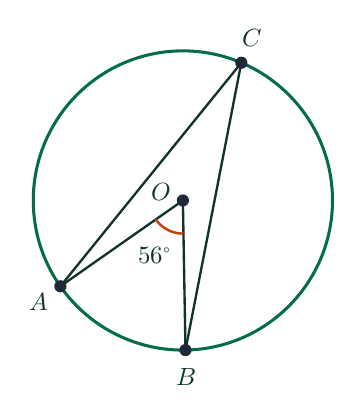
\begin{tikzpicture}
\draw[color={rgb,255:red,4;green,107;blue,77}, line width=1.1pt] (0,0) circle (1.900);
\draw[ink, line width=0.85pt] (0.742,1.749) -- (-1.556,-1.090);
\draw[ink, line width=0.85pt] (0.742,1.749) -- (0.033,-1.900);
\draw[ink, line width=0.85pt] (0.000,0.000) -- (-1.556,-1.090);
\draw[ink, line width=0.85pt] (0.000,0.000) -- (0.033,-1.900);
\draw[color={rgb,255:red,194;green,65;blue,12}, line width=0.9pt] (-0.344,-0.241) -- (-0.332,-0.257) -- (-0.319,-0.273) -- (-0.305,-0.289) -- (-0.291,-0.303) -- (-0.276,-0.317) -- (-0.260,-0.330) -- (-0.243,-0.342) -- (-0.226,-0.354) -- (-0.209,-0.364) -- (-0.191,-0.374) -- (-0.172,-0.383) -- (-0.153,-0.391) -- (-0.134,-0.398) -- (-0.114,-0.404) -- (-0.094,-0.409) -- (-0.074,-0.413) -- (-0.054,-0.417) -- (-0.034,-0.419) -- (-0.013,-0.420) -- (0.007,-0.420);
\node[font=\small, text=ink, inner sep=0.5pt, fill=white] at (-0.354,-0.695) {$56^\circ$};
\fill[color={rgb,255:red,31;green,41;blue,55}] (-1.556,-1.090) circle (2.2pt);
\fill[color={rgb,255:red,31;green,41;blue,55}] (0.033,-1.900) circle (2.2pt);
\fill[color={rgb,255:red,31;green,41;blue,55}] (0.742,1.749) circle (2.2pt);
\fill[color={rgb,255:red,31;green,41;blue,55}] (0.000,0.000) circle (2.2pt);
\node[font=\small, text=ink, inner sep=0.5pt] at (-1.835,-1.285) {$A$};
\node[font=\small, text=ink, inner sep=0.5pt] at (0.039,-2.240) {$B$};
\node[font=\small, text=ink, inner sep=0.5pt] at (0.875,2.062) {$C$};
\node[font=\small, text=ink, inner sep=0.5pt] at (-0.282,0.103) {$O$};
\end{tikzpicture}
\end{document}
